\documentclass{article}

% Language setting
% Replace `english' with e.g. `spanish' to change the document language
\usepackage[english]{babel}

% Set page size and margins
% Replace `letterpaper' with `a4paper' for UK/EU standard size
\usepackage[letterpaper,top=2cm,bottom=2cm,left=3cm,right=3cm,marginparwidth=1.75cm]{geometry}

% Useful packages
\usepackage{amsmath}
\usepackage{graphicx}
\usepackage{subcaption} % For subfigures
\usepackage[colorlinks=true, allcolors=blue]{hyperref}
\usepackage{float}

\title{Machine Learning Exercise 0}
\author{Amélie Assmayr (12007770) \and
        Konstantinos Damanakis (12106343) \and
        Teresa Schuch (12007762)}

\begin{document}
\maketitle

\section{Introduction}

In this Exercise we have chosen two datasets: Laptop Prices and Road Traffic Accidents. The Laptop Prices dataset will be utilized to develop models for predicting laptop prices based on various specifications, while the Road Traffic Accidents dataset will be employed to classify the severity of accidents in the capital city of Ethiopia. \newline

We decided on those two datasets because they enable us to try various and diverse techniques within our framework as they cover different aspects. The Laptop Prices dataset is clean, with no missing values, and consists of 15 features. On the other hand, the Road Traffic Accidents dataset contains 20.057 missing values in 16 variables and includes over 30 features, making the preprocessing steps for this dataset more important and complex.

\section{Dataset 1: Laptop Prices}

The Laptop Price dataset contains information about various laptops and their prices in Euros. It includes detailed specifications that describe each laptop's features and capabilities. With this we aim to build a machine learning model that can predict laptop prices based on these specifications. \newline

We chose the Laptop Price dataset because of its importance in real-life situations. Most people today rely on laptops for work, education and entertainment. Understanding these prices can help consumers make informed purchasing decisions, making this dataset highly relevant in today’s technology-driven world. Additionally, the variety of features in the dataset, including both categorical and numeric data makes it ideal for experimenting with feature engineering and different machine learning methods.

\subsection{Attribute Types}

The dataset has 2275 instances and 15 variables. The variables together with their datatypes can be seen in the table below:

\begin{table}[H]
    \parbox{.40\linewidth}{
        \begin{tabular}{l|r}
            \textbf{Variable} & \textbf{Datatype} \\\hline
            Company & nominal \\
            Product & nominal \\
            Type Name & nominal \\
            Inches & ratio quantity \\
            Screen Resolution & ordinal \\
            CPU Company & nominal \\
            CPU Type & nominal \\
            CPU Frequency (GHz) & ratio quantity
        \end{tabular}
}
    \hfill
    \parbox{.40\linewidth}{
        \begin{tabular}{l|r}
            \textbf{Variable} & \textbf{Datatype} \\\hline
            RAM (GB) & ratio quantity \\
            Memory & ordinal \\
            GPU Company & nominal \\
            GPU Type & nominal \\
            Operating System & nominal \\
            Weight (kg) & ratio quantity \\
            Price (Euro) & ratio quantity 
        \end{tabular}}
        
\end{table}

This results in 8 nominal variables, 2 ordinal variables and 5 metric variables. A key advantage of this dataset is the absence of missing values across all variables, eliminating the need for additional preprocessing steps in this regard.

\subsection{Target attribute}
The target variable is the price of the laptop. Accurately estimating this price—potentially through regression analysis—can provide retailers with crucial insights into expected revenues before official pricing is announced. The histogram below illustrates the distribution of laptop prices, revealing that most laptops are priced between 400 and 800 €. However, the mean price stands at 1135 €, with a median of 989 €. Calculating the median makes sense since we can see that there a a few laptops that cost between 5000 and 6000 € which is much higher than the rest. Still these outliers are valid values. The prices range between 174€ and 6099€.

\begin{figure}[H]
\centering
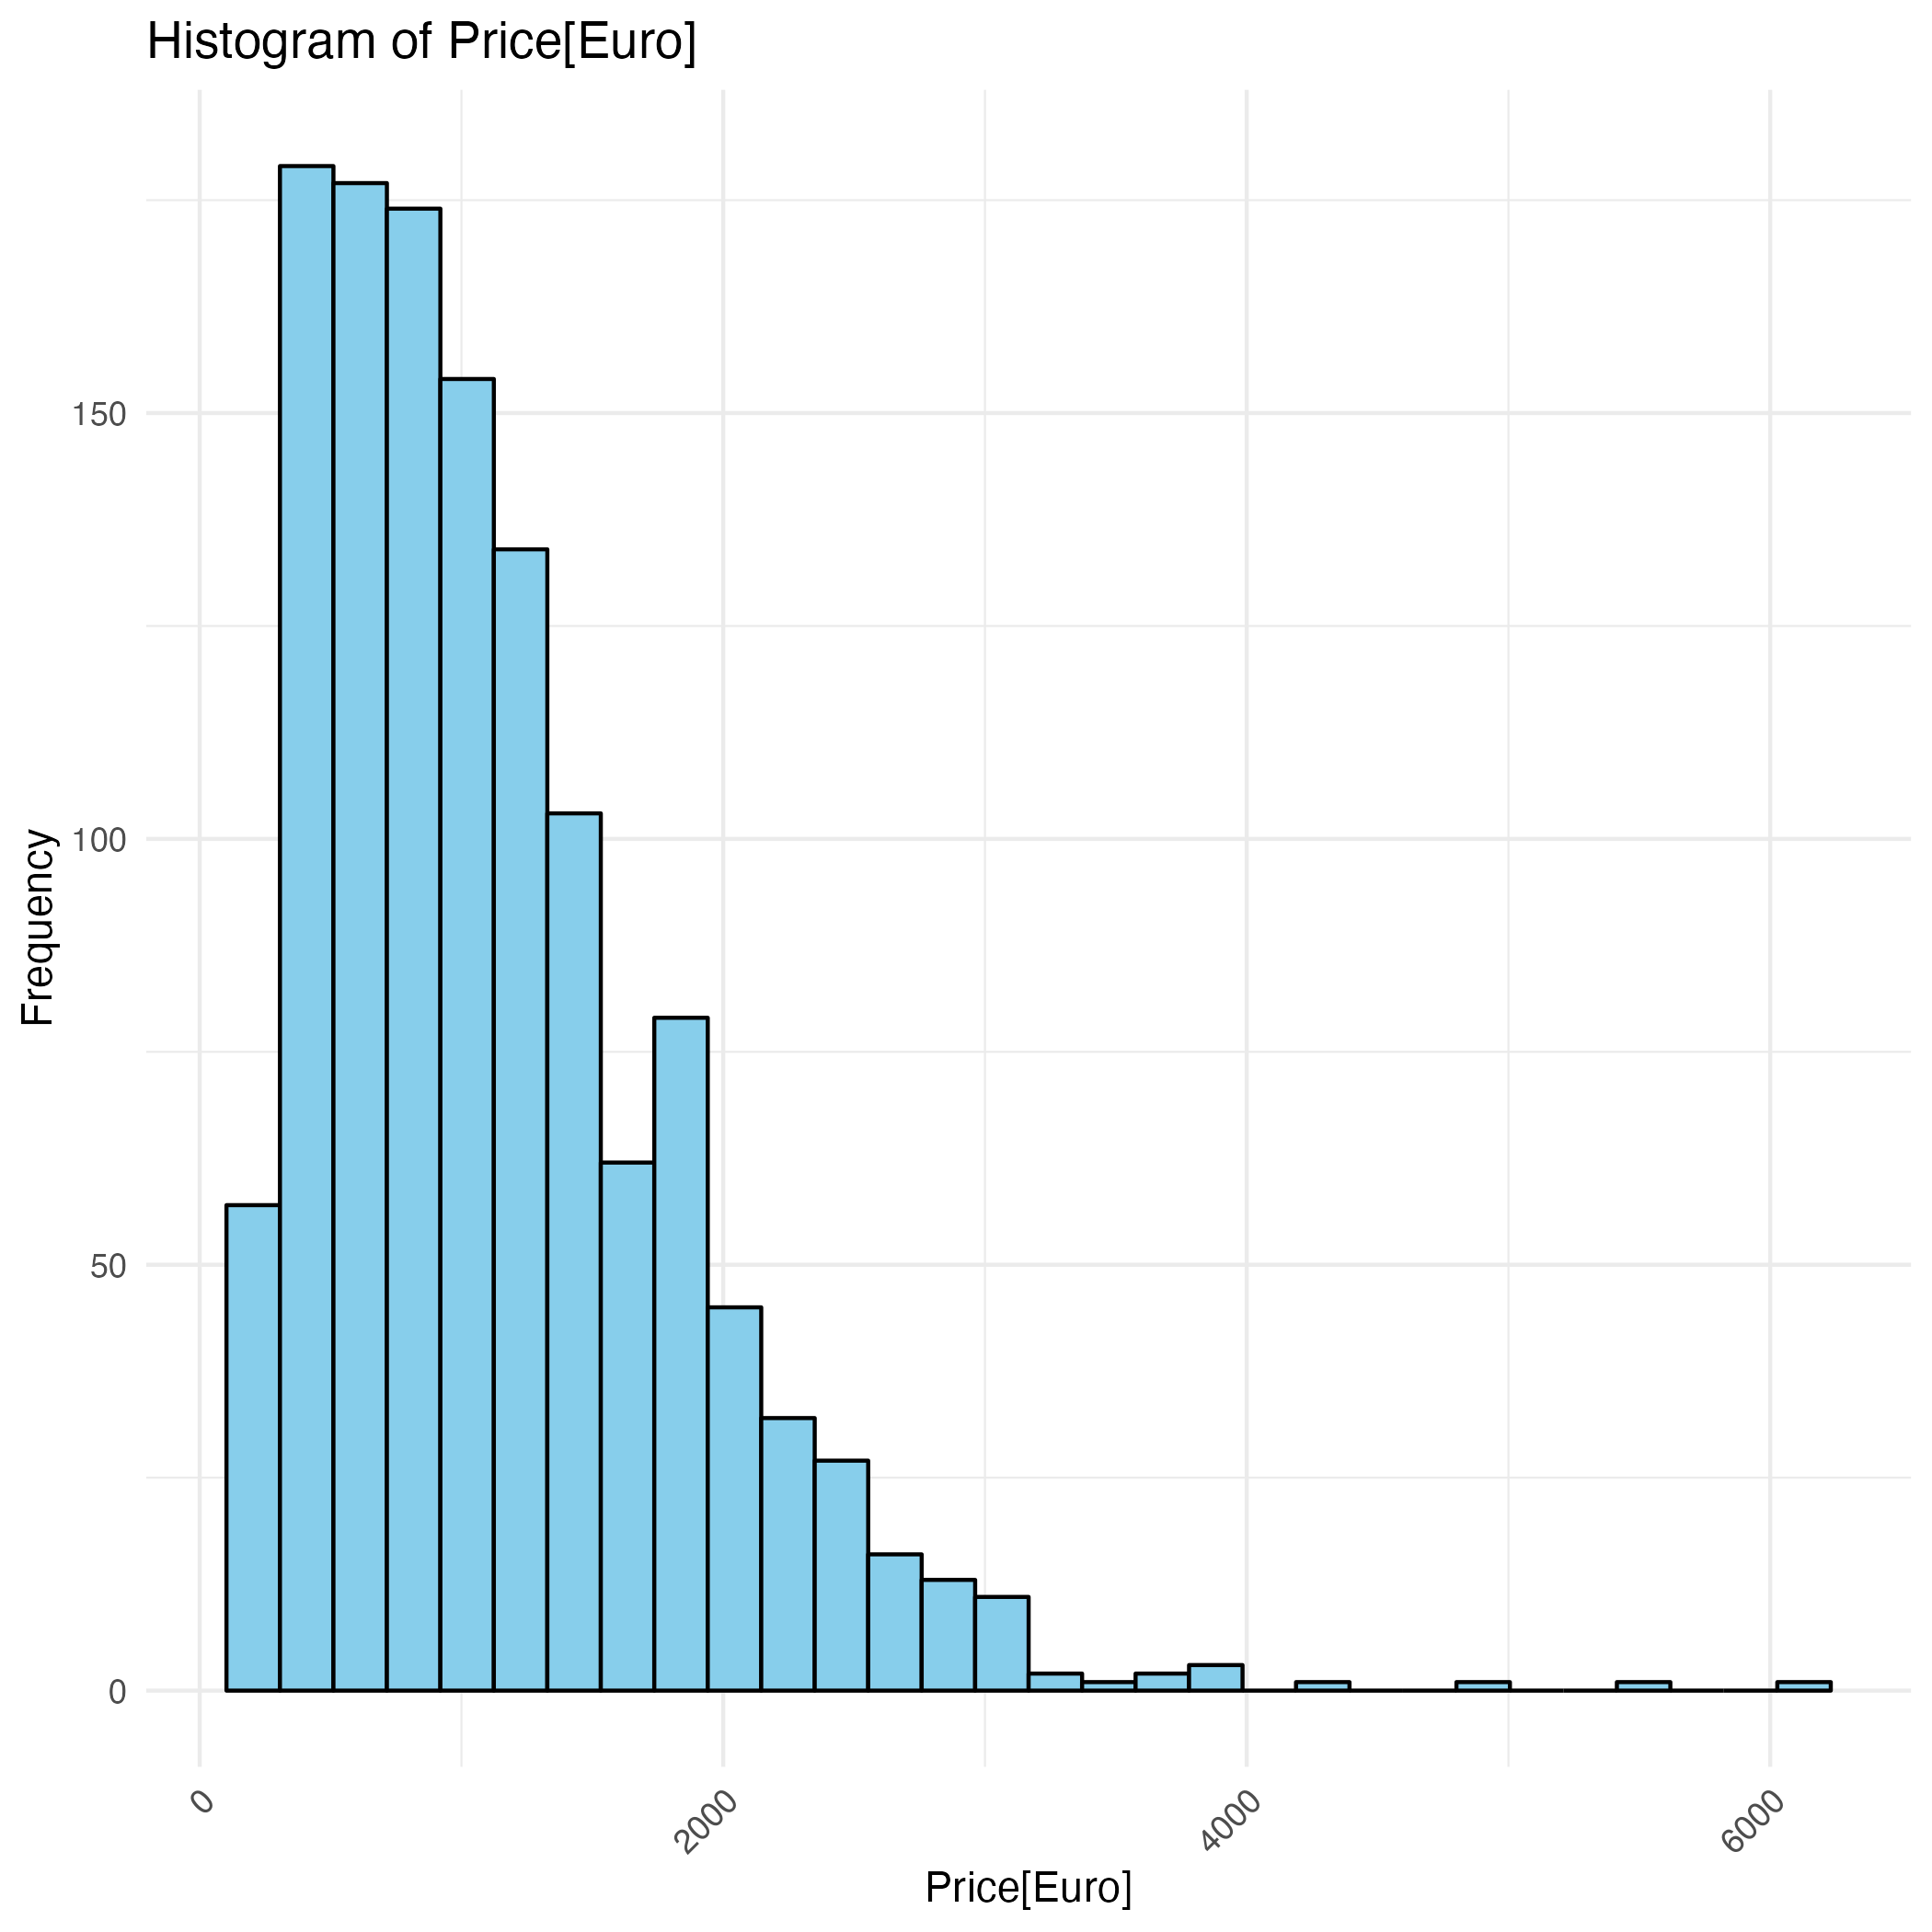
\includegraphics[width=0.5\linewidth]{Histogram_Price.png}
\caption{\label{fig:hist:price}Histogramm Laptop Price}
\end{figure}

\subsection{Additional Attribute Insights}
\subsubsection{Numeric attributes}

\begin{itemize}
    \item \textbf{Screen Size:} Ranges from 10.10 to 18.40 inches, with a mean of 15.02 inches.
    \item \textbf{Weight:} Varies between 0.690 kg and 4.7 kg, with an average weight of 2.041 kg.
    \item \textbf{CPU Frequency:} Spans from 0.9 to 3.6 GHz, with a mean value of 2.5 GHz.
    \item \textbf{RAM:} Takes integer values between 2 and 64 GB, with a median value of 8 GB.
\end{itemize}

In the plot below the distribution of the screen size and the RAM can be seen as an example.

\begin{figure}[H]
    \centering
    \begin{subfigure}[b]{0.45\textwidth}
        \centering
        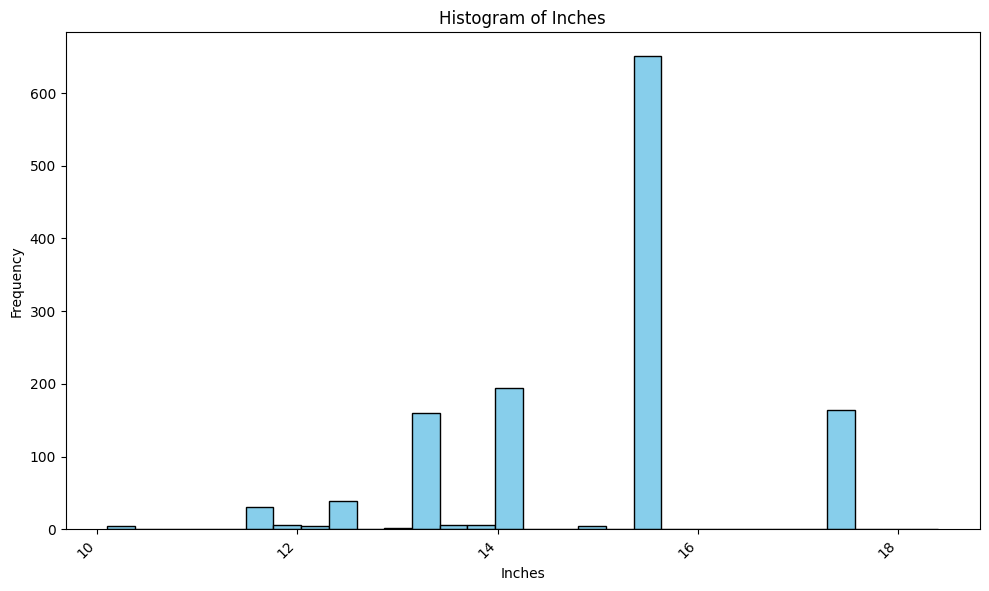
\includegraphics[width=\linewidth, height=5cm]{Histogram_Inches.png} 
        \caption{Histogram Inches}
        \label{fig:figure1}
    \end{subfigure}
    \hspace{0.05\textwidth} % Adjust space between figures
    \begin{subfigure}[b]{0.45\textwidth}
        \centering
        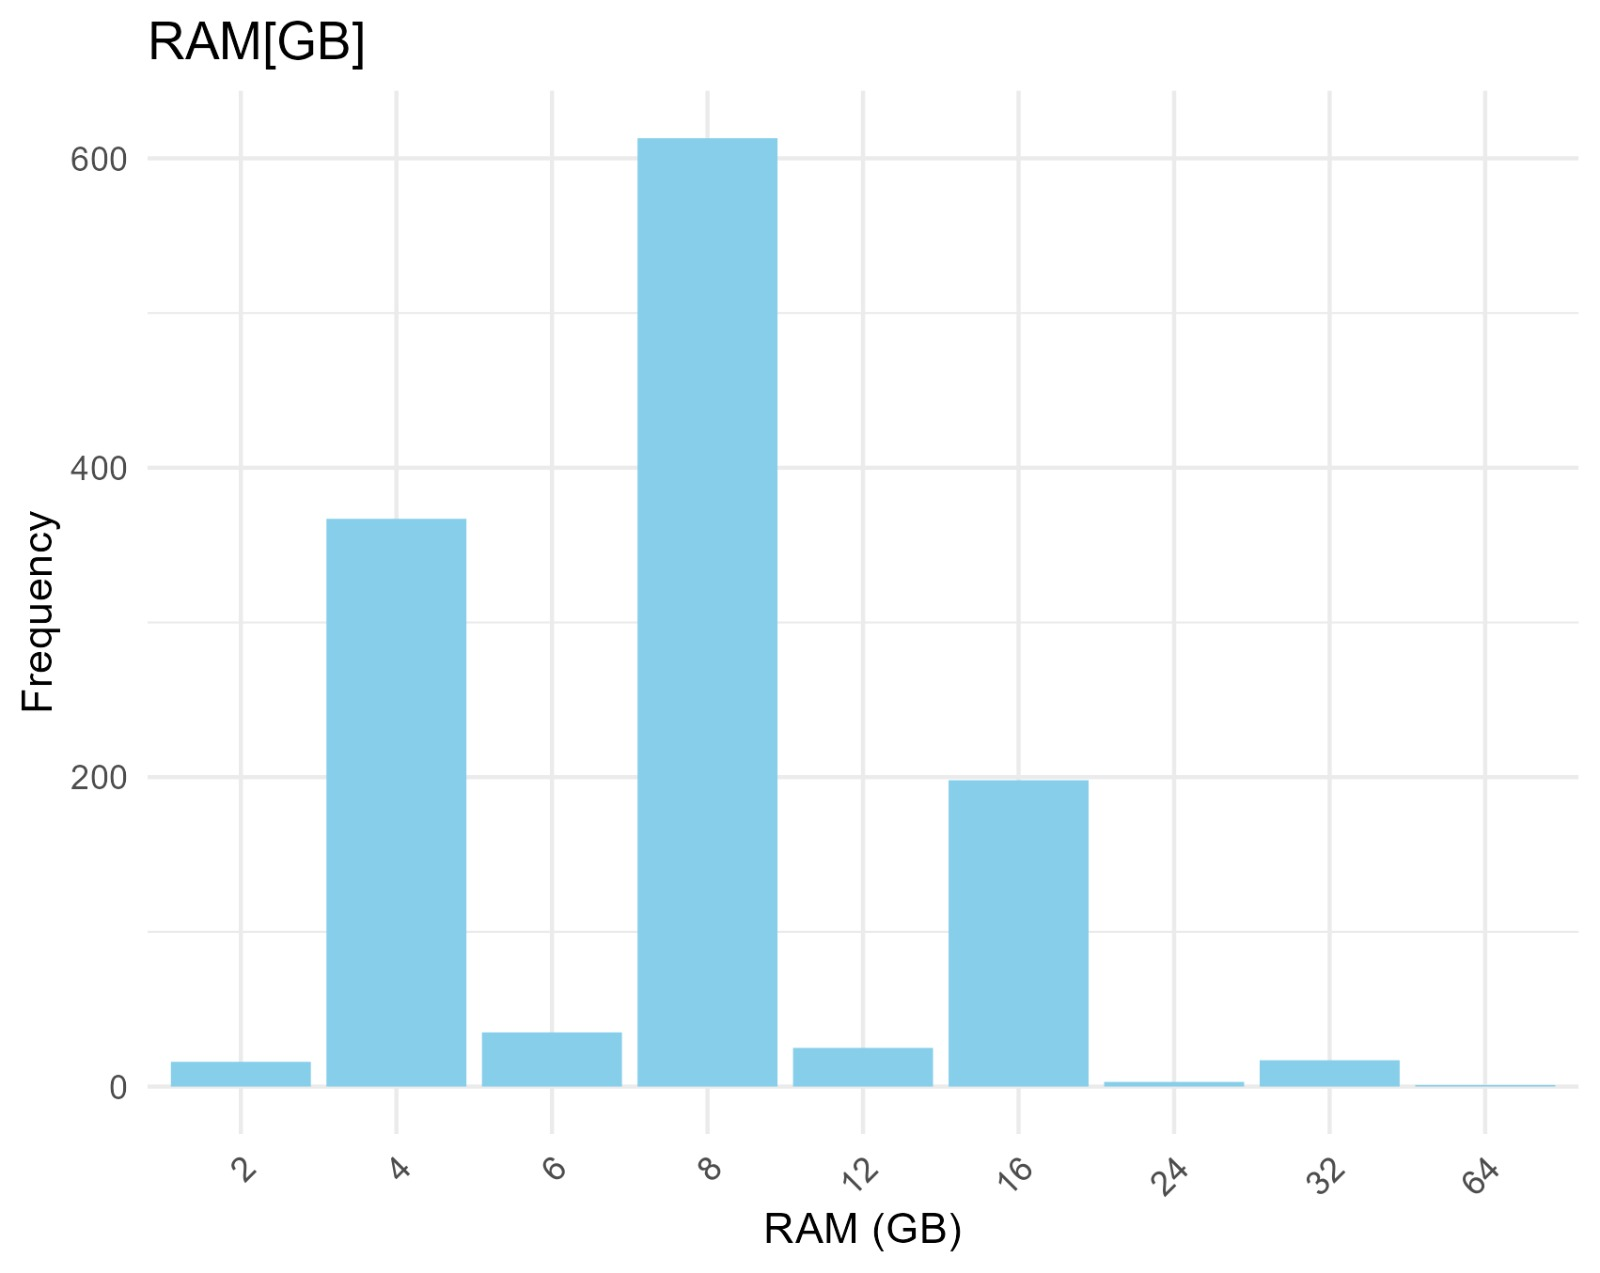
\includegraphics[width=\linewidth]{Barplot_RAM.jpeg} 
        \caption{Histogram RAM}
        \label{fig:figure2}
    \end{subfigure}
    \label{fig:two_figures}
\end{figure}

\subsubsection{categorical attributes}

For categorical variables, we assessed the number of distinct values. 

\begin{table}[H]
    \centering
    \begin{tabular}{|c|c|c|c|c|}
        \hline
        \textbf{Company} & \textbf{Product} & \textbf{TypeName} & \textbf{ScreenResolution} & \textbf{CPU\_Company} \\ \hline
        19 & 618 & 6 & 40 & 3 \\ \hline
        \textbf{CPU\_Type} & \textbf{Memory} & \textbf{GPU\_Company} & \textbf{GPU\_Type} & \textbf{OpSys}       \\ \hline
        93 & 39 & 4 & 106 & 9 \\ \hline
    \end{tabular}
    \caption{Laptop Dataset Features}
    \label{tab:laptop_features}
\end{table}

The variable product may require preprocessing due to its numerous unique values, which could complicate regression analysis. It could be possible to summarize some variables e.g. Vostro 3559, Vostro 3568, Vostro 5370, Vostro 5468, Vostro 5471 Vostro 5568 could all be merged to just Vostro. \newline

As an example there are two barplots below of the Company and the CPU Type. Given that especially the CPU Type has many distinct values, only the top 10 values are represented to maintain clarity in visualization.

\begin{figure}[H]
    \centering
    \begin{subfigure}[b]{0.45\textwidth}
        \centering
        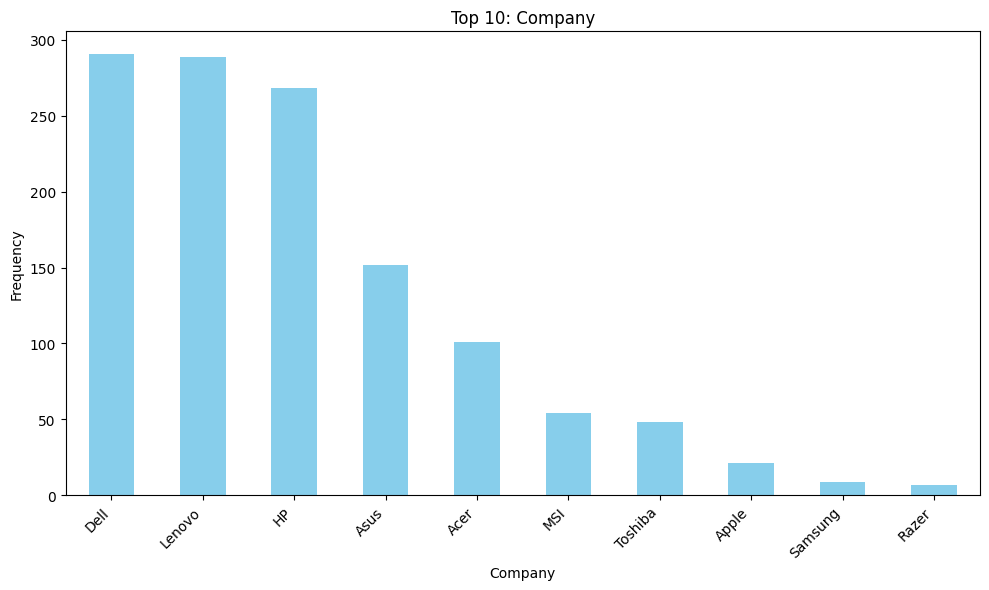
\includegraphics[width=\linewidth]{Barplot_Company.png} 
        \caption{Barplot Company}
        \label{fig:figure1}
    \end{subfigure}
    \hspace{0.05\textwidth} % Adjust space between figures
    \begin{subfigure}[b]{0.45\textwidth}
        \centering
        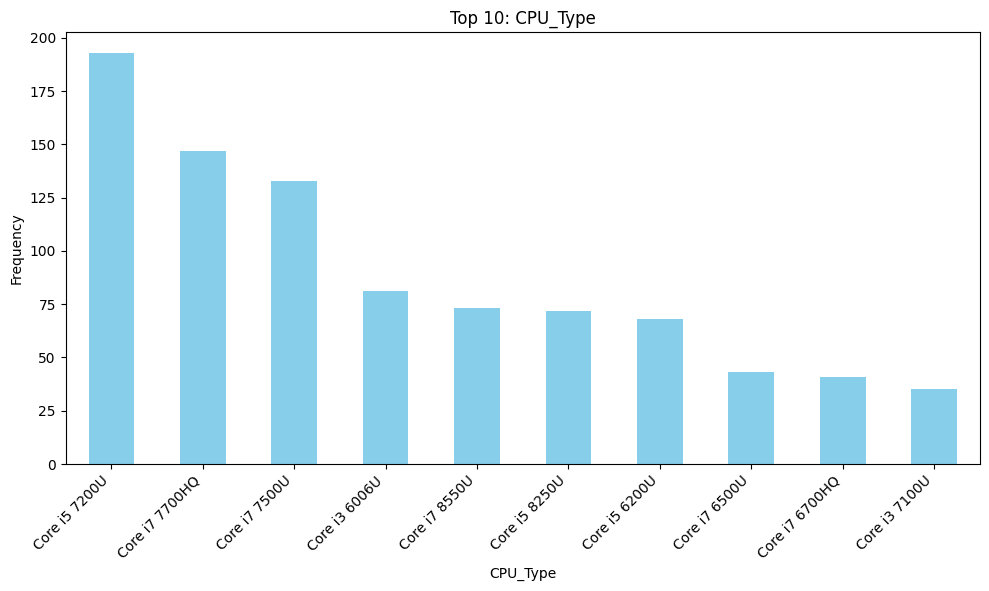
\includegraphics[width=\linewidth]{Barplot_CPUTypes.png} 
        \caption{Barplot CPU Types}
        \label{fig:figure2}
    \end{subfigure}
    \label{fig:two_figures}
\end{figure}


\section{Dataset 2: Road Traffic Accidents}

The Road Traffic Accidents dataset includes instances of road traffic accidents recorded in the years between 2017 and 2020 in Addis Ababa, capital city of Ethiopia. This dataset contains information regarding the number and the characteristics of the vehicles and the drivers that took part in the accidents, the conditions and the casualties that happened as a result of these unfortunate events.\newline

We chose this dataset because it addresses a critical public safety issue that affects many people. A study of this data and a development of a machine learning model would enable the classification and prediction of the severity of the accident based on the different features that lead to or are involved in the accident. This analysis can help identify the major causes and factors contributing to road safety, which is essential for improving transportation policies and reducing accidents. 

\subsection{Attribute Types}

The data contain 31 attributes related to the accident and the target variable which is the severity of the accident. There are 12316 samples/cases recorded while missing data can be observed in 16 of the 32 features.  In the following table all 31 attributes are presented together with their type of data:

\begin{table}[H]
    \parbox{.40\linewidth}{
        \begin{tabular}{l|r|c}
            \textbf{Variable} & \textbf{Datatype} &
            \textbf{Unique}\\\hline
            Time & ratio quantity & / \\
            Day of Week & nominal & 7\\
            Age of Driver & ratio quantity & /\\
            Sex of Driver & nominal & 3\\
            Educational Level & nominal &7\\
            Vehicle-Driver Relation & nominal & 4 \\
            Driving Experience & ratio quantity & /\\
            Vehicle Type & nominal & 17\\
            Vehicle Owner & nominal & 4\\
            Vehicle Service Year & ratio quantity & /\\
            Defect of Vehicle & nominal & 3 \\
            Accident Area & nominal & 14\\
            Lanes or Medians & nominal & 7\\
            Road Alignment & nominal & 9\\
            Junction Type & nominal & 8\\
            Road Surface Type & nominal  & 4
        \end{tabular}
}
    \hfill
    \parbox{.40\linewidth}{
        \begin{tabular}{l|r|c}
            \textbf{Variable} & \textbf{Datatype} &
            \textbf{Unique}\\\hline
            Road Surface Condition & nominal & 4\\
            Light Condition & nominal & 4 \\
            Weather Condition & nominal & 9\\
            Collision Type & nominal & 10 \\
            Number of Vehicles & ratio quantity & /\\
            Number of Casualty & ratio quantity & /\\
            Vehicle Movement & nominal & 13 \\
            Casualty Class & nominal & 4\\
            Sex of Casualty & nominal & 3 \\
            Age of Casualty & ratio quantity & /\\
            Casualty Severity & ordinal & 4 \\
            Work of Casualty & nominal & 7\\
            Fitness of Casualty & nominal & 5 \\
            Pedestrian Movement & nominal & 9\\
            Cause of Accident & nominal & 20\\
            Severity of Accident & nominal & 3
        \end{tabular}}
\end{table}

This results in 24 nominal variables, 1 ordinal variable and 7 metric variables. Preprocessing steps are necessary to handle the missing values.

\subsection{Target Attribute}

The target variable is the severity of the accident. It is classified into the three following classes: Light Injury, Serious Injury or Fatal Injury. While the severity could be considered an ordinal variable, we will treat it as nominal, framing the task as a multiclass classification problem. The following plot shows the distribution of these classes. It can be seen that the classes are really unevenly distributed. Most accidents fall under the "Slight Injury" category, with 10,415 instances, followed by "Serious Injury" with 1,743 instances, and only 158 accidents classified as "Fatal Injury." This imbalance is a critical factor to consider when developing and evaluating the model.

\begin{figure}[H]
\centering
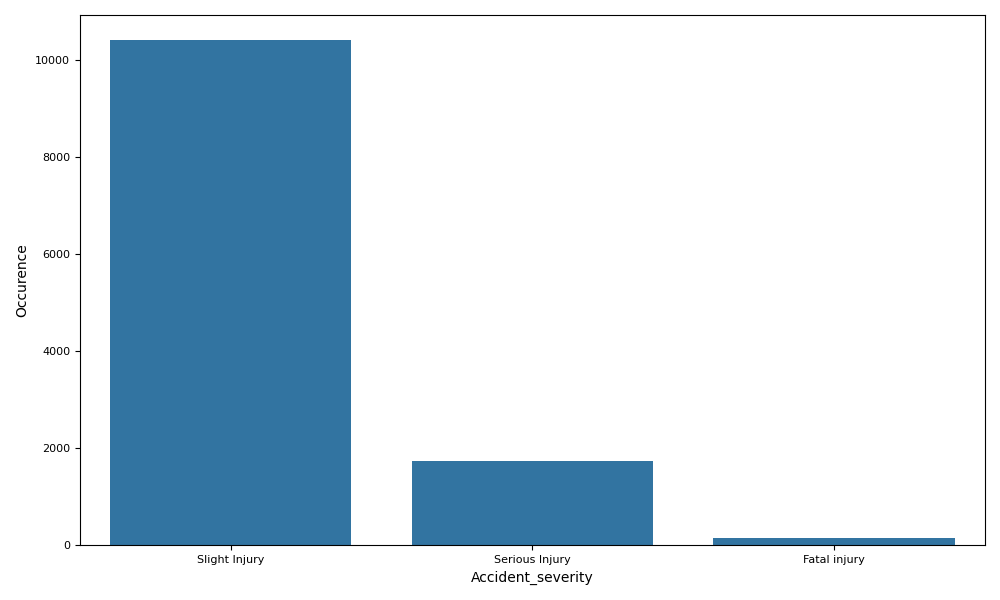
\includegraphics[width=0.5\linewidth]{Accident_severity.png}
\caption{\label{fig:hist:price}Barplot Accident Severity}
\end{figure}

\subsection{additional attribute insights}

\subsubsection{numerical variables}

Most of the numeric variables in the dataset are grouped into intervals, effectively converting them into ordinal data. For instance, Driving Experience is categorized into intervals such as: below 1 year, 1-2 years, 2-5 years, 5-10 years, above 10 years, and no license. In fact only the time, the number of Vehicles and the number of Casualty remain as numeric variables. \newline

ToDo: insert plots

\subsubsection{categorical variables}

The number of unique values for each categorical variable can be seen in the table 3. There are no variable with more than 20 categories so there is no need to merge multiple categories into on or applying similar techniques. \newline

ToDo: insert plots

\subsubsection{other interesting insights}
The table below shows the number of missing values in the respective columns. 

\begin{table}[H]
    \parbox{.40\linewidth}{
        \begin{tabular}{l|r|c}
            \textbf{Column} & \textbf{Missing Values} \\\hline
            Educational Level & 741 \\
            Vehicle Driver Relation & 579\\
            Driving Experience & 829\\
            Vehicle Type & 950\\
            Vehicle Owner & 482\\
            Vehicle Service Year & 3.928\\
            Vehicle Defect & 4.427\\
            Accident Area & 239\\
        \end{tabular}
}
    \hfill
    \parbox{.40\linewidth}{
        \begin{tabular}{l|r|c}
           \textbf{Column} & \textbf{Missing Values} \\\hline
            Lanes or Medians & 385 \\
            Road Alignment & 142\\
            Junction Type & 887\\
            Road Surface Type & 172\\
            Collision Type & 155\\
            Vehicle Movement & 308\\
            Work Casuality & r3.198\\
            Fitness Casuality & 2.635\\
        \end{tabular}}
\end{table}

Besides regular missing values, the dataset has other entries like 'Unknown' or 'na' that represent missing or unclear data. These should be handled during preprocessing to improve data quality and model accuracy.

\end{document}